%
% This is a borrowed LaTeX template file for lecture notes for CS267,
% Applications of Parallel Computing, UCBerkeley EECS Department.
% Now being used for CMU's 10725 Fall 2012 Optimization course
% taught by Geoff Gordon and Ryan Tibshirani.  When preparing 
% LaTeX notes for this class, please use this template.
%
% To familiarize yourself with this template, the body contains
% some examples of its use.  Look them over.  Then you can
% run LaTeX on this file.  After you have LaTeXed this file then
% you can look over the result either by printing it out with
% dvips or using xdvi. "pdflatex template.tex" should also work.
%
\documentclass[twoside]{article}
\usepackage{graphicx}
\usepackage{tikz}
\usepackage{hyperref}
\hypersetup{colorlinks=true, citecolor=blue, filecolor=blue, linkcolor=blue, urlcolor=blue}
\usetikzlibrary{decorations.pathmorphing}

\setlength{\oddsidemargin}{0.25 in}
\setlength{\evensidemargin}{-0.25 in}
\setlength{\topmargin}{-0.6 in}
\setlength{\textwidth}{6.5 in}
\setlength{\textheight}{8.5 in}
\setlength{\headsep}{0.75 in}
\setlength{\parindent}{0 in}
\setlength{\parskip}{0.1 in}
%
% ADD PACKAGES here:
%
\usepackage{amsmath,amsfonts,graphicx}
%
% The following commands set up the lecnum (lecture number)
% counter and make various numbering schemes work relative
% to the lecture number.
%
\newcounter{lecnum}
\renewcommand{\thepage}{\thelecnum-\arabic{page}}
\renewcommand{\thesection}{\thelecnum.\arabic{section}}
\renewcommand{\theequation}{\thelecnum.\arabic{equation}}
\renewcommand{\thefigure}{\thelecnum.\arabic{figure}}
\renewcommand{\thetable}{\thelecnum.\arabic{table}}
%
% The following macro is used to generate the header.
%
\newcommand{\lecture}[5]{
   \pagestyle{myheadings}
   \thispagestyle{plain}
   \newpage
   \setcounter{lecnum}{#1}
   \setcounter{page}{1}
   \noindent
   \begin{center}
   \framebox{
      \vbox{\vspace{2mm}
    \hbox to 6.28in { {\bf Physics 467/667: Thermodynamics/Statistical Physics
	\hfill Spring 2017} }
       \vspace{4mm}
       \hbox to 6.28in { {\Large \hfill Lecture #1: #2  \hfill} }
       \vspace{2mm}
       \hbox to 6.28in { {\it Lecturer: #3 \hfill Scribes: #4} }
      \vspace{2mm}}
   }
   \end{center}
   \markboth{Lecture #1: #2}{Lecture #1: #2}
   \vspace*{4mm}
}
%
% Convention for citations is authors' initials followed by the year.
% For example, to cite a paper by Leighton and Maggs you would type
% \cite{LM89}, and to cite a paper by Strassen you would type \cite{S69}.
% (To avoid bibliography problems, for now we redefine the \cite command.)
% Also commands that create a suitable format for the reference list.
\renewcommand{\cite}[1]{[#1]}
\def\beginrefs{\begin{list}%
        {[\arabic{equation}]}{\usecounter{equation}
         \setlength{\leftmargin}{2.0truecm}\setlength{\labelsep}{0.4truecm}%
         \setlength{\labelwidth}{1.6truecm}}}
\def\endrefs{\end{list}}
\def\bibentry#1{\item[\hbox{[#1]}]}
%Use this command for a figure; it puts a figure in wherever you want it.
%usage: \fig{NUMBER}{SPACE-IN-INCHES}{CAPTION}
\newcommand{\fig}[3]{
			\vspace{#2}
			\begin{center}
			Figure \thelecnum.#1:~#3
			\end{center}
	}
% Use these for theorems, lemmas, proofs, etc.
\newtheorem{theorem}{Theorem}[lecnum]
\newtheorem{lemma}[theorem]{Lemma}
\newtheorem{proposition}[theorem]{Proposition}
\newtheorem{claim}[theorem]{Claim}
\newtheorem{corollary}[theorem]{Corollary}
\newtheorem{definition}[theorem]{Definition}
\newenvironment{proof}{{\bf Proof:}}{\hfill\rule{2mm}{2mm}}
% **** IF YOU WANT TO DEFINE ADDITIONAL MACROS FOR YOURSELF, PUT THEM HERE:
\newcommand\E{\mathbb{E}}
\begin{document}
%FILL IN THE RIGHT INFO.
%\lecture{**LECTURE-NUMBER**}{**DATE**}{**LECTURER**}{**SCRIBE**}
%\lecture{6}{The Second Law and Entropy}{Qiang Zhu}{scribe-name1,2,3}
%\footnotetext{These notes are partially based on those of Nigel Mansell.}
% **** YOUR NOTES GO HERE:
% Some general latex examples and examples making use of the
% macros follow.  
%**** IN GENERAL, BE BRIEF. LONG SCRIBE NOTES, NO MATTER HOW WELL WRITTEN,
%**** ARE NEVER READ BY ANYBODY.

\section*{Homework}
\begin{enumerate}
\item Write a code to calculate $\Omega(N)$ in the context of flipping coins and plot them when $N$=10, 15, 30, 100.
\begin{figure}[h]
\centering
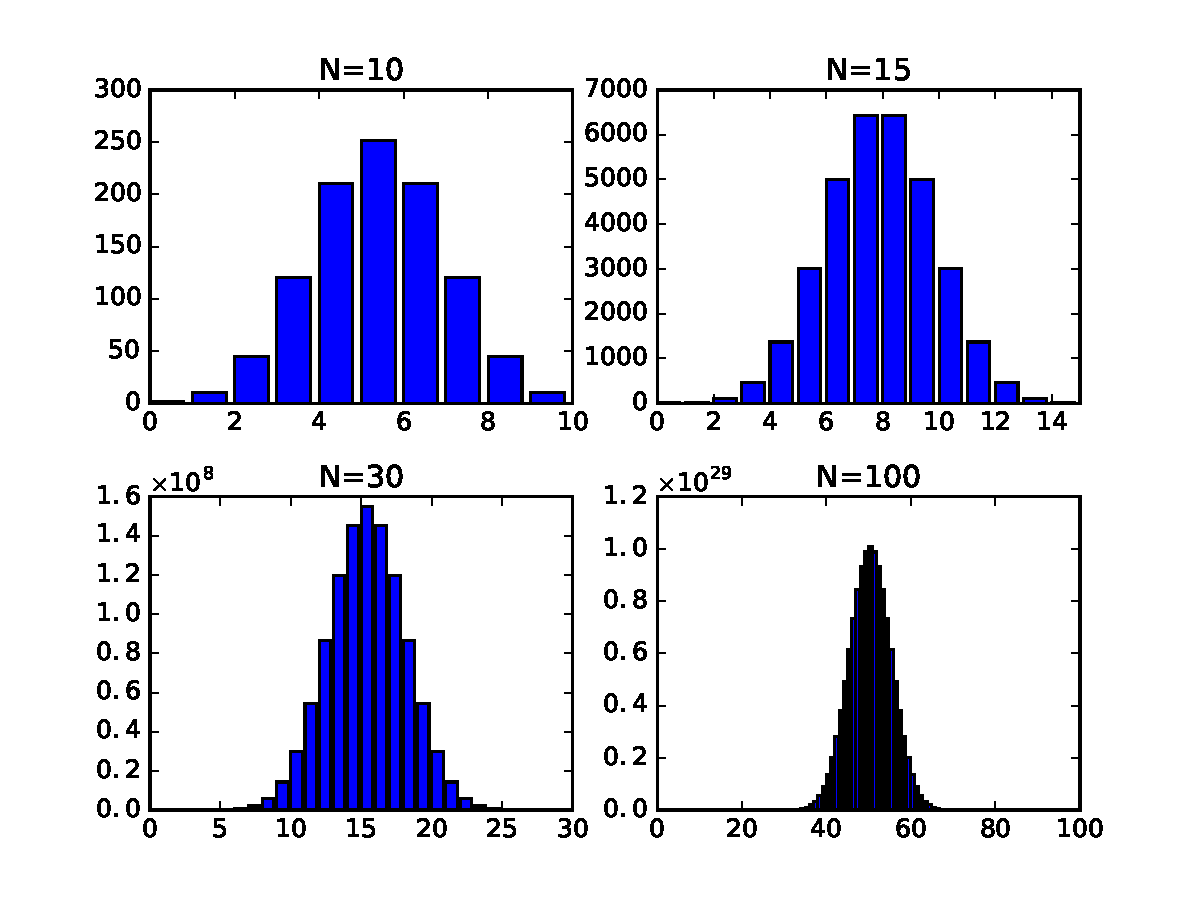
\includegraphics[width=9cm]{imgs/flip}
\caption{The number of $\Omega$ as a function of $N$ in the game of flipping coins. }
\end{figure}



\item Write a code to calculate $\Omega(N)$ in the context of Einstein solid and plot them when $N$=10, 15, 30, 100 and $q$ from 0 to 10.
\begin{figure}[h]
\centering
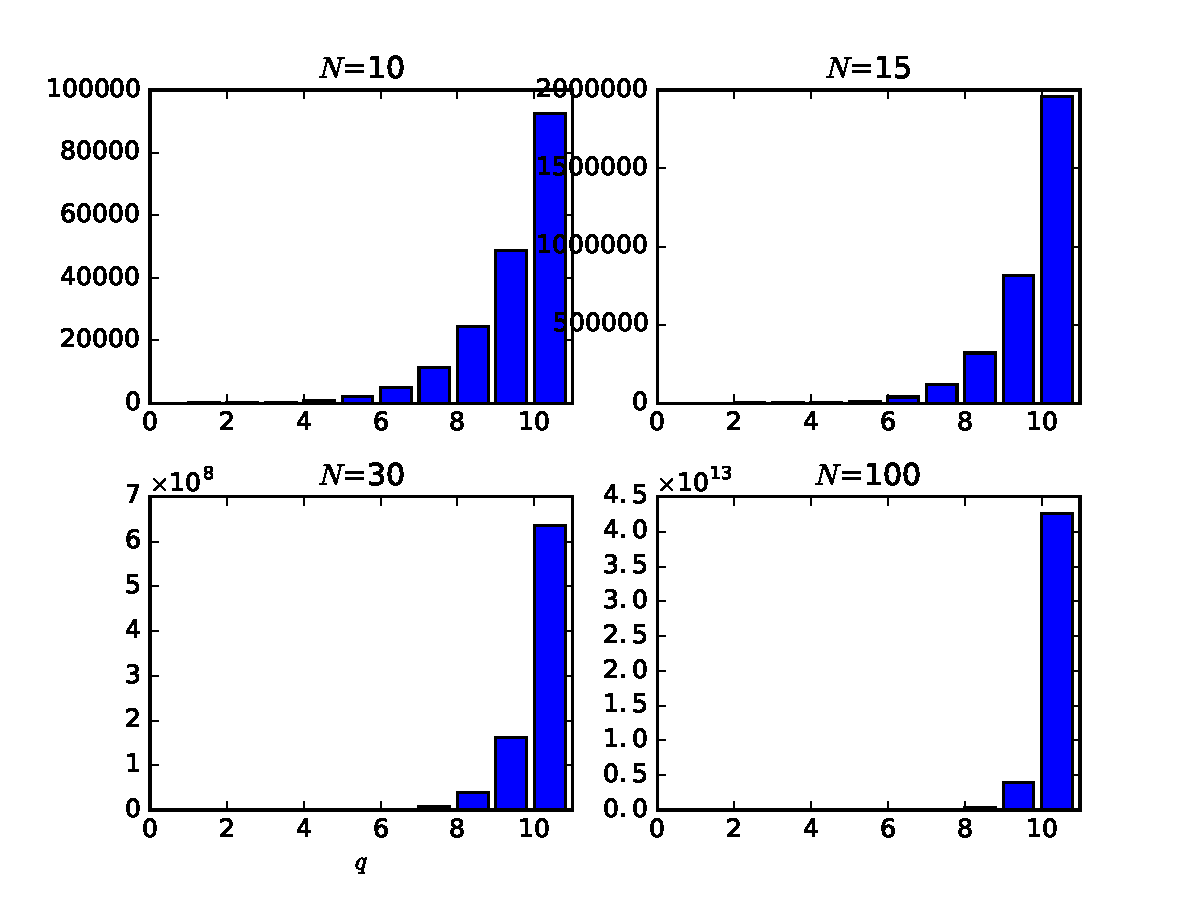
\includegraphics[width=10cm]{imgs/Einstein0}
\caption{The number of $\Omega$ as a function of $N$ in an Einstein solid. }
\end{figure}

\item Write a code to calculate $\Omega$ as a function of $q_A$, when $N_A$=[300, 600, 3000, 6000], $N_B$=[200, 400, 2000, 4000],
and $q$=100, plot them and try to find some tendency when $N$ increases (hint: 4 plots).
\begin{figure}[h]
\centering
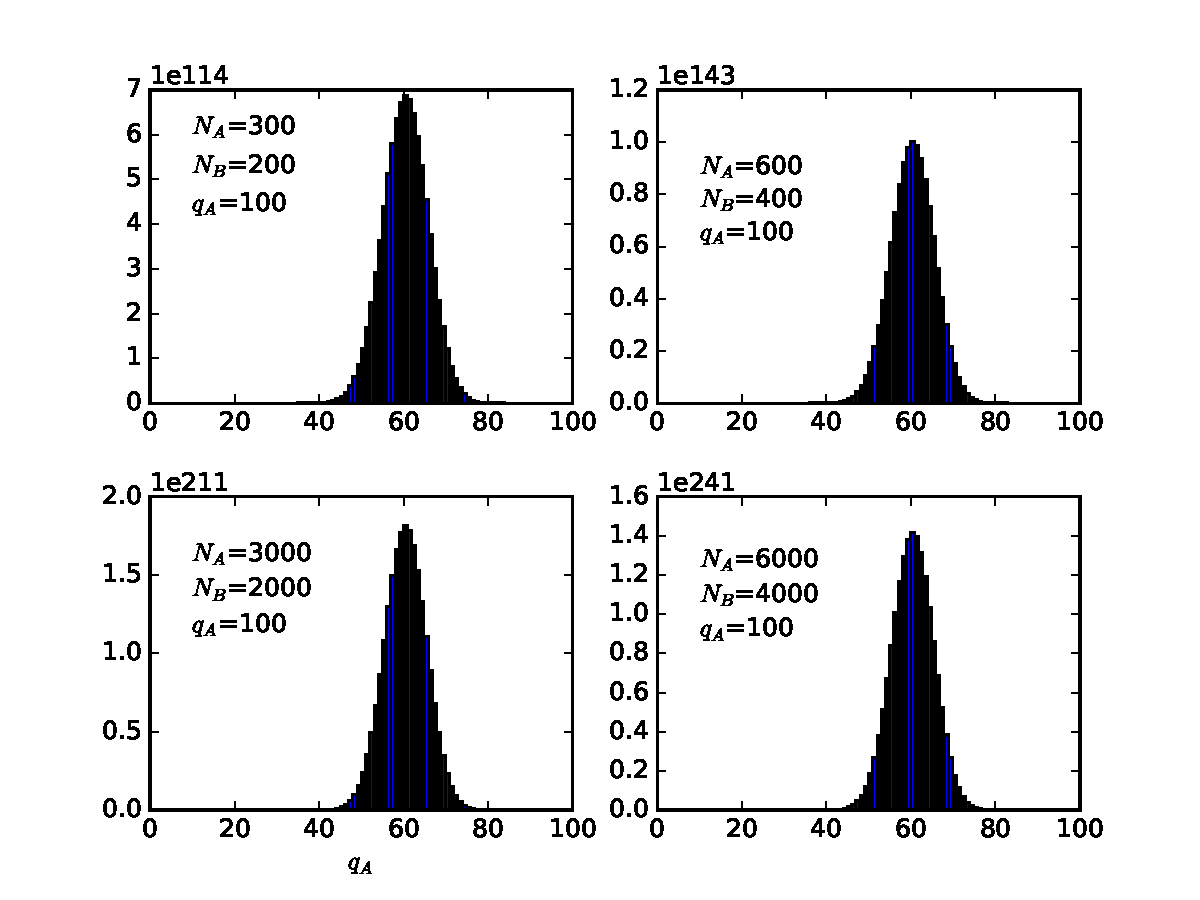
\includegraphics[width=10cm]{imgs/Einstein.pdf}
\caption{$\Omega$ as a function of $N$ in two interacting Einstein solids. }
\end{figure}

\item Write a code to calculate the probability of $\Omega(q_A)$, when $N_A$=[300, 3000], $N_B$=[200, 2000],
for $q$=[100, 1000], plot them and try to explain the differences. (hint: 2 plots)

\begin{figure}[h]
\centering
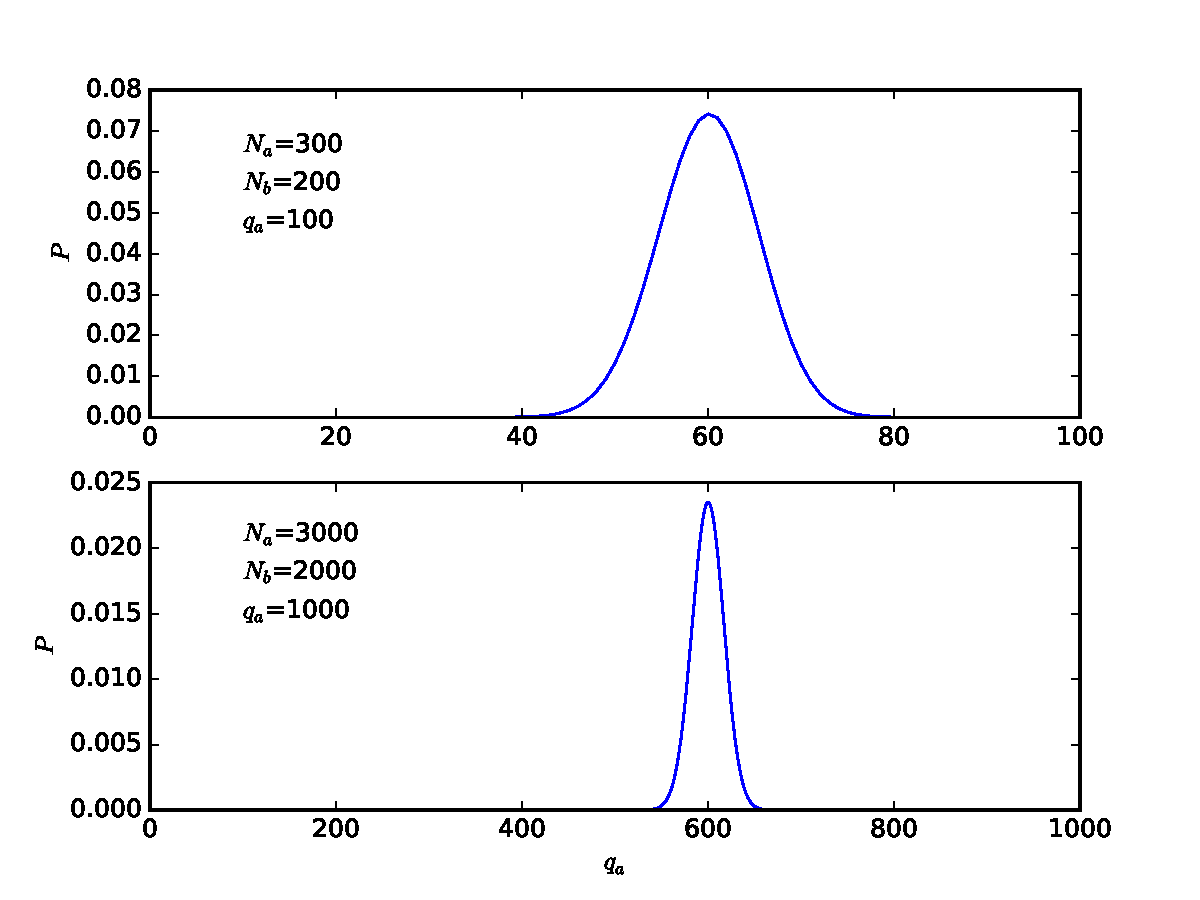
\includegraphics[width=9cm]{imgs/Einstein2.pdf}
\caption{Probability distribution of $\Omega(N)$ in two interacting Einstein solids for different $q$ values. }
\end{figure}

\end{enumerate}


\end{document}
